\documentclass{ctexart}
\usepackage[margin=1in]{geometry}
\usepackage{graphicx}
\begin{document}
\section{浮力调节}
\subsection{基本概念}
\paragraph{}为克服不同水域的温度、密度等因素的差异对AUV航行造成的影响,AUV上搭载浮力调节装置可使其具备更好的适应性。
\paragraph{}可调压载调节是指在AUV外形基本不变的情况下,通过改变AUV重量,使其所受重力与浮力的差值发生变化,而得到理想的受力状态。通常,采用的方法是在AUV中增加耐压水舱,通过海水泵配合阀组吸入或排出水舱中的水来改变AUV在水中的重量。
\paragraph{}可变体积调节是指在不改变AUV重量的情况下,采取调整排水体积的方式来改变其所受浮力的大小。通常采用的方法是在AUV内、外部分别安装2个经液压管路联通的油囊。当需要增加浮力时,系统液压泵配合相应的阀组将内油囊中的油抽排至外油囊,以增大外油囊的体积;当需要减小浮力时,系统将外油囊中的油抽回至内油囊,以减小外油囊的体积。
\subsection{浮力调节装置构成及工作原理}
\paragraph{}结合AUV的外形结构特点,使用浮力调节装置替换原有的艏、艉垂直槽道控制器和推进器。浮力调节装置在AUV上的布局位置如图1所示。AUV内部的电池组可以为装置的运行提供电能,AUV驾驶单元负责通过通信总线对装置下达控制指令以完成相应的调节功能。
\paragraph{}浮力调节装置结构设计为一个独立舱段。该装置舱段总长720 mm,自重96 kg,舱段壳体采用5A06铝合金材料,在舱段外部,使用过渡支架将外油囊固定于原有的垂向槽道内,并经穿壁油管使其与舱段中的内油囊相连。如此安装,既可利用槽道空腔对外油囊进行保护,又能够减小对原有AUV外形的改变程度,确保了在航行期间不产生额外阻力。舱段内部的液压和电子设备分别安装在隔板的上、下部位,这样,既可节省空间,也能够减小不同类型设备间运行时产生的相互干扰。浮力调节舱段如下图所示:\\
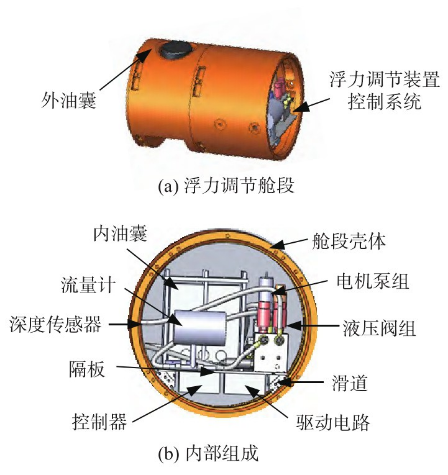
\includegraphics[scale=1]{./fulitiaojie.png}
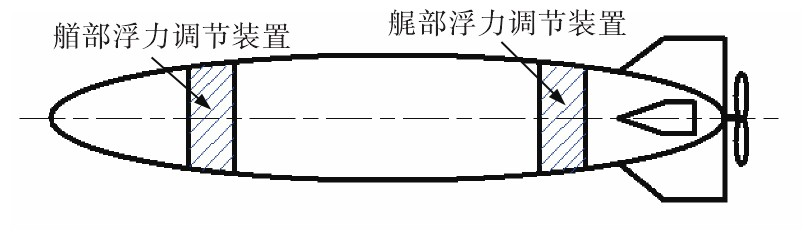
\includegraphics[scale=1.6]{./fulitiaojie2.png}
\clearpage
\subsection{计算过程}
\paragraph{}AUV体积: 
\[V=3.14\times 0.25^2 \times 2=0.3925m^3\]
浮力:
\[F=\rho gV=1.025\times 10^3\times 10\times 0.3925=4023N \]
舱体在空气中的重量约为:$300Kg$,24小时内吸水重量:
\[200Kg\times 1\%=20Kg\]
\end{document}